\documentclass[usenames,dvipsnames]{beamer}
% * <formanek@vse.cz> 2018-04-02T11:05:51.176Z:
%
% ^.
%
% Choose how your presentation looks.
%
\usepackage[T1]{fontenc}
\usepackage[utf8]{inputenc}
\usepackage{lmodern}  
\usepackage{tikz}%boxy  
\usetikzlibrary{arrows,positioning}
\usetikzlibrary{calc}
\usepackage{amsmath}
\usepackage{bm}
\usepackage{graphicx}
\usepackage{color}
\usepackage{hyperref}
%
% For more themes, color themes and font themes, see:
% http://deic.uab.es/~iblanes/beamer_gallery/index_by_theme.html
%
\mode<presentation>
{
  \usetheme{Darmstadt}      % or try Darmstadt, Madrid, Warsaw, ...
  \usecolortheme{default} % or try albatross, beaver, crane, ...
  \usefonttheme{serif}  % or try default, serif, structurebold, ...
  \setbeamertemplate{navigation symbols}{}
  \setbeamertemplate{caption}[numbered]
  \setbeamertemplate{headline}{}
}
%
% 
%
\newcommand{\mytikzmark}[2]{%
  \tikz[remember picture,inner sep=0pt,outer sep=0pt,baseline,anchor=base] 
    \node (#1) {\ensuremath{#2}};}
%
%
\newcommand*\circled[1]{\tikz[baseline=(char.base)]{
    \node[shape=circle,draw=Red,inner sep=2pt] (char) {#1};}}
%
\newcommand*\circledd[1]{\tikz[baseline=(char.base)]{
    \node[shape=circle,draw=ProcessBlue, dashed, inner sep=2pt] (char) {#1};}}
%
%
\newcommand*{\boxcolor}{Red}
\makeatletter
\renewcommand{\boxed}[1]{\textcolor{\boxcolor}{%
\tikz[baseline={([yshift=-1ex]current bounding box.center)}] \node [rectangle,semithick, minimum width=1ex,draw, dashed] {\normalcolor\m@th$\displaystyle#1$};}}
 \makeatother
%
%
%
\title[Week6]{Week 6: Panel data \& methods}
\author{Advanced Econometrics 4EK608}
\institute{Vysoká škola ekonomická v Praze}
\date{}

\begin{document}
 
\begin{frame}
  \titlepage
\end{frame}

% Uncomment these lines for an automatically generated outline.
\begin{frame}{Content}
  \tableofcontents
\end{frame}

%---------------------------------
\section{Pooled cross sections}
\begin{frame}{Pooled cross sections}
\begin{itemize}
\item \underline{\textbf{Pooled cross sections data:}}
Random sampling from a large population at different time periods. For example: 400 randomly selected respondents in a survey, 5 consecutive years. For each year, we have a different - randomly chosen - set of respondents. 
\item Pooled cross sections should not be confused with “actual” panel data (where we would follow individual respondents across time). 
\item Pooled cross sections: sampling from a changing population at different points in time generates \textbf{independent, not identically distributed} (\textit{inid}) observations. 
\item Pooled cross sections are easy to deal with, simply by allowing the intercept (and perhaps some selected slopes) in a LRM to vary across time. 
\item Can be used for policy analysis (difference-in-differences estimator). 
\end{itemize}
\end{frame}
%---------------------------------
\begin{frame}{Pooled cross sections}
\underline{\textbf{Pooled cross sections - model example}}
\begin{align*}
\log(\textit{wage}_{it}) & = \theta_0 + \theta_1 d91_t + \theta_2 d92_t + \delta_1 \textit{female}_{it} + \delta_2 \textit{educ}_{it} +\\
& + \gamma_1 \textit{exper}_{it} + \gamma_2 (\textit{female} \times d91)_{it} + \gamma_3 (\textit{female} \times d92)_{it} + u_{it} 
\end{align*}
\medskip
where $t = 1990, 1991, 1992$; \hspace{0.2cm} $i=1,2, \dots , \mytikzmark{500}{500}$ \\
$d91_{t}$ and $d92_t$ are time dummies, \\
\vspace{0.2cm}
$\textit{female}_{it}$, $\textit{educ}_{it}$ and $\textit{exper}_{it}$ describe the gender, education and work experience of the $i$-th individual at time $t$, \\
\vspace{0.2cm}
$(\textit{female} \times d91)_{it}$ is an interaction element, may be used to describe whether changes in wages over time are statistically different for man and woman.
\begin{tikzpicture}[<-,overlay,remember picture,inner sep=1.5pt,shorten <=0.2em,font=\tiny]
\tikzset{
    mynode/.style={rectangle,draw=ProcessBlue, fill=White, semithick, inner sep=.2em, minimum size=2em, text centered, text width=8em},
    myarrow/.style={->, >=stealth, thin, Red}
}
\node[mynode] at (4.7,3.3) (Box){Each year, we draw $500$ individuals at random. Individual respondents are not followed. Total observations: $N \times T = 1.500$};
  \draw[myarrow] (Box) -- ++   (500);
\end{tikzpicture}
\end{frame}
%---------------------------------
\begin{frame}{Pooled cross sections: Chow test}
\underline{\textbf{Pooled cross sections - model example contd.}}
\begin{align*}
 \log(\textit{wage}_{it}) =  \beta_0 & + \beta_1 d91_t + \beta_2 d92_t + \beta_3 \textit{female}_{it} + \\
 & + \beta_4 \textit{educ}_{it} + \beta_5 \textit{exper}_{it} + u_{it}
\end{align*}
\textbf{Chow test for structural changes across time} \\
\smallskip
Basically an \textit{F}-test for linear restrictions, can be used to determine whether the estimated slope coefficients change across time.\\
\medskip
In our $\log(wage)$ equation, we would test the $H_0$ of ``time-invariant'' $\beta_3, \beta_4$ and $\beta_5$ coefficients, while allowing for time dummies (time-specific intercepts).
\end{frame}
%---------------------------------
\begin{frame}{Pooled cross sections: Chow test}
\vspace{1cm}
\vfill
\bigskip
$F=\frac{( \mytikzmark{SSRr}{\textit{SSR}_r}- \mytikzmark{SSRur}{\textit{SSR}_{ur}}}{\textit{SSR}_{ur}} \cdot \frac{(n-T-Tk)}{(T-1)k};$ \\
\bigskip
{\small under $H_0$ of no structural break, $F \sim F((T-1)k, (n- \mytikzmark{TTk}{\circledd{$T-Tk$)}})$} \\
\bigskip
\begin{itemize}
\item [Note:] This test is not robust to heteroskedasticity (including changing variance across time). Robust variants of the test exist, based on interaction terms.
\end{itemize}
\begin{tikzpicture}[<-,overlay,remember picture,inner sep=1.5pt,shorten <=0.2em,font=\scriptsize]
\tikzset{
    mynode/.style={rectangle,draw=ProcessBlue, dashed, fill=White, semithick, inner sep=.2em, minimum size=2em, text centered, text width=9em},
    myarrow/.style={->, >=stealth, thin, ProcessBlue}
}
\node[mynode] at (1,6.2) (SSRr*){$\textit{SSR}_r$: restricted model – pooled regression, allowing for different time intercepts.};
\draw[myarrow] (SSRr*) -- ++   (SSRr);
	\node[mynode] at (5.5,6.2) (SSRur*){$\textit{SSR}_{ur}$:run a regression for each of the time periods. $\textit{SSR}_{ur} = 			\textit{SSR}_1 + \textit{SSR}_2 + \dots + \textit{SSR}_T$};
	\draw[myarrow] (SSRur*) -- ++   (SSRur);
		\node[mynode] at (9.3,6.2) (TTk*){$T + Tk$ parameters estimated in the unrestricted model};
		\draw[myarrow] (TTk*) -- ++   (TTk);
\end{tikzpicture}
\end{frame}
%---------------------------------
% Define box and box title style
\tikzstyle{mybox} = [draw=blue!35, fill=white, very thick,
    rectangle, rounded corners, inner sep=1pt, inner ysep=10pt]
\tikzstyle{fancytitle} =[fill=blue!35, text=black]
%---------------------------------
\section{Policy analysis with pooled cross sections (DiD estimator)}
\begin{frame}{Policy analysis with pooled cross sections}
\begin{tikzpicture}
\node [mybox] (box){%
\begin{minipage}{0.50\textwidth}
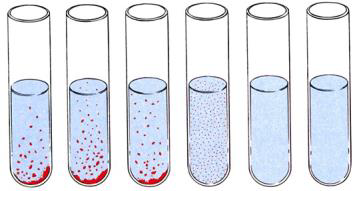
\includegraphics[width=\textwidth, height=2.89cm]{./img/Obrazek1}
\begin{itemize}
\scriptsize
\item Test tubes identical except for catalyst
\item Measure: Effect at different catalyst volumes (reaction speed, product volume, \dots)
\item Perform the experiment $n$-times
\item Control for other factors (heat, \dots)
\item Estimate average effect \\(\& standard error)
\end{itemize}
\end{minipage}
};
\node[fancytitle, right=5pt,  rounded corners] at (box.north west) {\scriptsize Scientific experiment};
\end{tikzpicture}%
\begin{tikzpicture}
\node [mybox] (box){%
\begin{minipage}{0.50\textwidth}
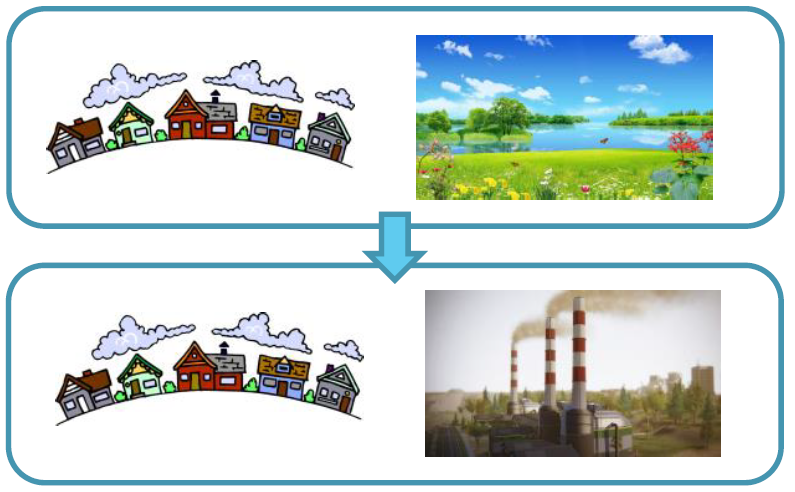
\includegraphics[width=\textwidth]{./img/Obrazek2}
\begin{itemize}
\scriptsize
\item Garbage incinerator is built in one given
suburban area over time
\item How do we estimate the effect on
individual house-prices?
\item Identical control group does not exist…
\item DiD: Difference-in-Differences estimator
(assumptions apply!)
\end{itemize}
\end{minipage}
};
\node[fancytitle, right=5pt,  rounded corners] at (box.north west) {\scriptsize Natural experiment (quasi-experiment)};
\end{tikzpicture}%
\end{frame}
%---------------------------------
\begin{frame}{Policy analysis with pooled cross sections}
\vfill
{\footnotesize \underline{\textbf{DiD example: In-house employee training for women}} \\
\underline{\textbf{returning from maternal leave \& its wage effect}}} \\
\medskip
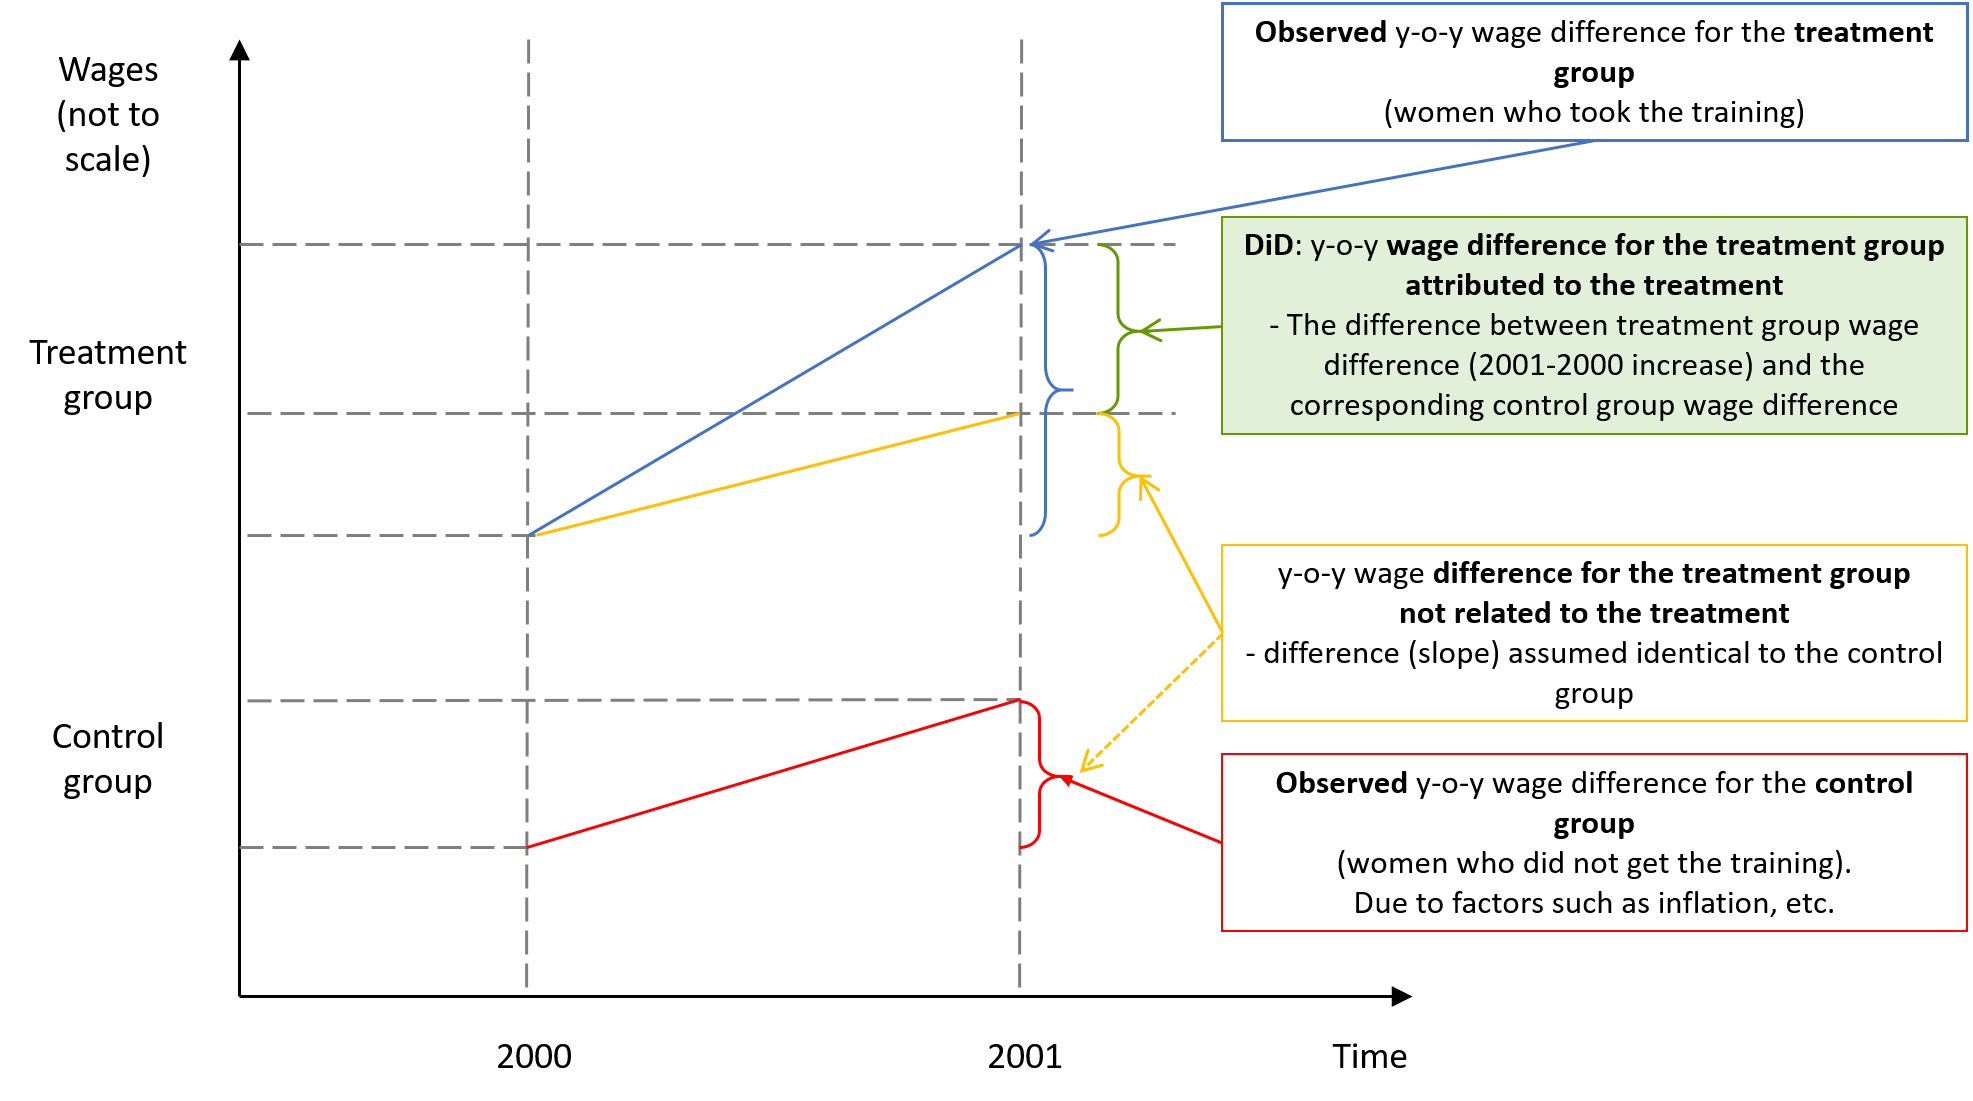
\includegraphics[width=\textwidth]{./img/Obrazek3}
\end{frame}
%---------------------------------
\begin{frame}{Policy analysis with pooled cross sections}
\underline{\textbf{DiD estimator:}} we can use LRMs to compare the changes in conditional means for the treatment and control groups…
\begin{itemize}
\item Group specific and time specific effects are allowed (controlled for)
\end{itemize}
\underline{\textbf{Assumptions:}}
\begin{itemize}
\item Unbiased DiD estimates require that the treatment (being subject to economic policy change…) is not systematically
related to factors affecting the outcome (dependent variable) that are not accounted for explicitly in our model and
thus are “hidden” in the random element.
\item DiD \textbf{attributes all differences in trends} between the treatment and control groups \textbf{to the intervention} (treatment). We assume there are no other factors that affect the difference in trends between the two groups.
\end{itemize}
\end{frame}
%---------------------------------
\begin{frame}{Example: policy analysis with pooled cross sections}
$y_{it}=\beta_0 + \delta_0 d2 + \beta_1 dT + \delta_1 (d2 \times dT) + \bm{x}_{it} \bm{\gamma} + u_{it},$\\
\medskip
$i=1, \dots, N;~~t=1,2$. \\
\bigskip
where:
\begin{itemize}
\item[$d2$] is a dummy variable, $d2=1$ for the second period (post treatment),
\item[$dT$] is a dummy variable, equals 1 for the individuals in the treatment group,
\item[$\bm{x}_{it}$ ] is a $1 \times k$ (row) vector of additional regressors and \\
$\bm{\gamma}$ is a $k \times 1$ vector of coefficients.
\end{itemize}
\end{frame}
%---------------------------------
\begin{frame}{Example: policy analysis with pooled cross sections}
$y_{it}=\beta_0 + \delta_0 d2 + \beta_1 dT + \delta_1 (d2 \times dT) + u_{it},$\\
\medskip
$i=1, \dots, N;~~t=1,2$. \\
\bigskip
In this simplified model (we drop $\bm{x}_{it} \bm{\gamma}$), the estimated $\delta_1$ \\has a convenient DiD interpretation:
\begin{align*}
\hat{\delta}_1 &= (\overline{y}_{Tr,\,t=2} - \overline{y}_{Co,\,t=2}) -  (\overline{y}_{Tr,\,t=1} - \overline{y}_{Co,\,t=1}), \\ ~& \\
& \hspace{0.5cm} \textnormal{which may be rearranged as:} \\ ~& \\
&= (\overline{y}_{Tr,\,t=2} - \overline{y}_{Tr,\,t=1}) -  (\overline{y}_{Co,\,t=2} - \overline{y}_{\textit{Co},\,t=1})
\end{align*}
\end{frame}
%---------------------------------
\begin{frame}{Example: policy analysis with pooled cross sections}
\footnotesize
\begin{table}
\centering
\caption{Illustration of the DiD estimator}
\label{Tab1}
\begin{tabular}{|l|c|c|c|}
\hline
\multicolumn{1}{|c|}{$E(y_{it} | d2, dT)$} & Before $(t = 1)$    & After $(t=2)$                             & After - Before        \\ \hline
Control                                    & $\beta_0$           & $\beta_0 + \delta_0$                      & $\delta_0$            \\ \hline
Treatment                                  & $\beta_0 + \beta_1$ & $\beta_0 + \delta_0 + \beta_1 + \delta_1$ & $\delta_0 + \delta_1$ \\ \hline
Treatment - Control                        & $\beta_1$           & $\beta_1 + \delta_1$                      & \circled{$\delta_1$}            \\ \hline
\end{tabular}
\end{table} 
Even if $\bm{x}_{it} \bm{\gamma}$ is added back to the equation, interpretation of $\delta_1$ remains essentially unchanged.
\begin{tikzpicture}[<-,overlay,remember picture,inner sep=1.5pt,shorten <=0.2em,font=\tiny]
\tikzset{
    mynode/.style={rectangle,draw=MidnightBlue, very thick, inner sep=.2em, minimum size=3.73em, text width=25.8em}
}
\node[mynode] at (1,2.25) (Ram){ };
\end{tikzpicture}
\end{frame}
%---------------------------------
\begin{frame}{Example: policy analysis with pooled cross sections}
\footnotesize{What is the effect of building garbage incinerator on housing prices?}
\scriptsize
\begin{table}[]
\centering
\label{Tab21}
\begin{tabular}{lclcc}
\multicolumn{3}{l}{Dependent Variable: RPRICE}                                          &                      & \multicolumn{1}{l}{}      \\
\multicolumn{3}{l}{Included observations: 321}                                          &                      & \multicolumn{1}{l}{}      \\
                                &                      & \multicolumn{1}{c}{}           &                      & \multicolumn{1}{l}{}      \\
\multicolumn{1}{c}{Variable}    & Coefficient          & \multicolumn{1}{c}{Std. Error} & t-Statistic          & \multicolumn{1}{l}{Prob.} \\
                                
                                & \multicolumn{1}{l}{} &                                & \multicolumn{1}{l}{} & \multicolumn{1}{l}{}      \\
\multicolumn{1}{c}{C}           & 82517.23             & \multicolumn{1}{c}{2726.910}   & 30.26034             & 0.0000                    \\
\multicolumn{1}{c}{Y81}         & 18790.29             & \multicolumn{1}{c}{4050.065}   & 4.639502             & 0.0000                    \\
\multicolumn{1}{c}{NEARINC}     & -18824.37            & \multicolumn{1}{c}{4875.322}   & -3.861154            & 0.0001                    \\
\multicolumn{1}{c}{Y81*NEARINC} & -11863.90            & \multicolumn{1}{c}{7456.646}   & -1.591051            & 0.1126                    \\
                                
                                & \multicolumn{1}{l}{} &                                & \multicolumn{1}{l}{} & \multicolumn{1}{l}{}      \\
R-squared                       & 0.173948             & \multicolumn{2}{l}{Mean dependent var}                & 83721.36                  \\
Adjusted R-squared              & 0.166131             & \multicolumn{2}{l}{S.D. dependent var}                & 33118.79                  \\
S.E. of regression              & 30242.90             & \multicolumn{2}{l}{Akaike info criterion}             & 23.48429                  \\
Sum squared resid               & 2.90E+11             & \multicolumn{2}{l}{Schwarz criterion}                 & 23.53129                  \\
Log likelihood                  & -3765.229            & \multicolumn{2}{l}{Hannan-Quinn criter.}              & 23.50306                  \\
F-statistic                     & 22.25107             & \multicolumn{2}{l}{Durbin-Watson stat}                & 1.557107                  \\
Prob(F-statistic)               & 0.000000             & \multicolumn{2}{l}{}                                  & \multicolumn{1}{l}{}     
\end{tabular}
\end{table}
\begin{tikzpicture}[<-,overlay,remember picture,inner sep=1.5pt,shorten <=0.2em,font=\footnotesize]
\tikzset{
    mynode/.style={rectangle,draw=MidnightBlue, fill=MidnightBlue!30, very thick, inner sep=.5em, minimum size=2em, text width=25em}
}
\node[mynode] at (7.8, 0.3) (Table){
\scriptsize{PRICE - house price in real terms (USD) \\ 
$Y81$ – dummy variable for $1981$, \ ($t=1978,1981$)\\
$1978$ – before ``rumors''~; $1981$ – incinerator operational \\
NEARINC – dummy for the treatment group}};
\end{tikzpicture}
\end{frame}
%---------------------------------
\begin{frame}{Example: policy analysis with pooled cross sections}
\small
Incinerator effect on prices example, contd: \\
\medskip
The model may be easily expanded by explanatory variables such as: \textit{HOUSE.AGE, ROOMS, AREA, LOT.AREA}, etc. and the DiD interpretation remains basically unchanged \dots
\begin{block}{Selection bias (treatment effect vs. selection bias) example:}
\small
\textbf{Assumption:} “Unbiased DiD estimates require that the treatment is not systematically related to factors affecting the outcome that are not explicitly accounted for.”  \\
\medskip
Say, we have a “poor neighborhood” with relatively old and small houses and low house-prices. For complex reasons, it suffers from a representation deficit within the local city council (as compared to other “rich neighborhoods”) and is therefore more likely to get the incinerator. \\
\medskip
We do not have variables to control for this factor $\rightarrow$ the DiD estimator may be severely biased 
\end{block}
\end{frame}
%---------------------------------
\begin{frame}{Policy analysis with pooled cross sections}
\textbf{Treatment effects}\\
\medskip
Topic not fully covered here, for detailed information see:\\
\medskip
\begin{itemize}
\item[1.] Wooldridge: Econometric analysis of C-S and panel data, chapter 21 Estimating Average Treatment Effects
\medskip
\item[2.] Greene: Econometric analysis, chapter 19.6
\medskip
\item[3.] Angrist, Pischke: Mostly Harmless Econometrics
\end{itemize}
\end{frame}
%---------------------------------
\section{Panel data}
\begin{frame}{Panel data}
\begin{itemize}
\item $N$ individual CS units are followed over $T$ time periods
\medskip
\item Short panels: $N \gg T$ \\
Working with short panels is similar to CS data analysis. If CS units are randomly drawn from a population and $T$ is small and fixed, then asymptotic analysis (properties) hold for arbitrary time dependence and distributional heterogeneity across time.
\medskip
\item Long panels: $T \gg N$ \\
Working with long panels is similar to time-series analysis. In TS analysis, stationarity \& weak dependency conditions apply. SURE (Seemingly Unrelated Regression Equation) approach can be used: for the regression equations (with identical regressor structure), we estimate contemporaneous error covariances and use this information to improve efficiency of the estimate (see Greene, chapter 10.2)
\end{itemize}
\end{frame}
%---------------------------------
\begin{frame}{Panel data}
\begin{itemize}
\item Large panel datasets: $T$ and $N$ large\\
Both CS and TS analysis assumptions apply, specialized estimators exist for large (heterogeneous) panels.\\Cointegrated series in panels: estimation and tests by Pesaran.
\bigskip
\item \textbf{Balanced panels:} obs. available for all $T$ on all CS units. Often assumed for simplicity of interpretation.
\smallskip
\item \textbf{Unbalanced panels:} mechanics of coefficient estimation do not differ. Model interpretation may require formal description of why the panel may be unbalanced. \\Problems may be caused by: 
\begin{itemize}
    \item \textbf{Sample selection bias:} with e.g. self-selection, coefficients can be be biased and inconsistent.
    \item \textbf{Attrition bias:} even if participants are randomly selected  at the beginning of observation, they often leave (medical study, school, etc.) on a non-random basis.   
\end{itemize}
\end{itemize}
\end{frame}
%---------------------------------
\begin{frame}{Panel data}
\textbf{Pooled regression with panel data: \\
\textit{Heterogeneity bias\\
(Similar principle as the Simpson's paradox) }}
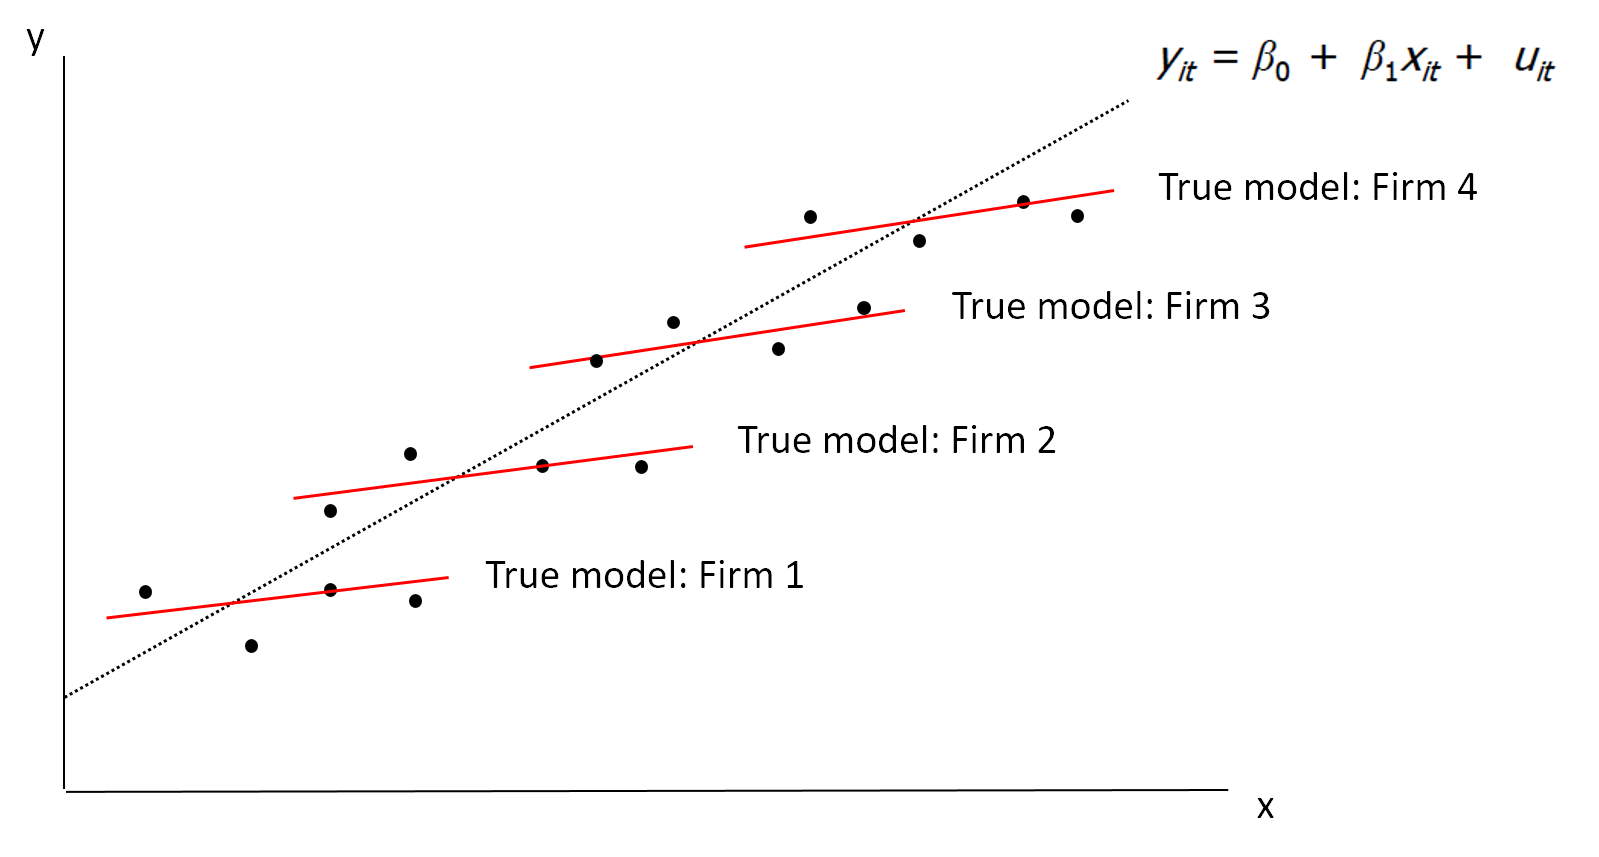
\includegraphics[width=\textwidth]{./img/Obrazek4}
\end{frame}
%---------------------------------
\begin{frame}{Panel data}
\textbf{Variation for the dependent variable and regressors}
\begin{itemize}
\item Overall variation: variation over time and individuals.
\item Between variation: variation between individuals.
\item Within variation: variation within individuals (over time).
\end{itemize}
\tiny
\begin{table}[]
\centering
\label{Tab3}
\noindent\makebox[\textwidth]{%
\begin{tabular}{|c|c|c|c|c|c|c|c|c|}
\hline
Id  & Time & Variable & \begin{tabular}[c]{@{}c@{}}Individual\\ mean\end{tabular} & \begin{tabular}[c]{@{}c@{}}Overall\\ mean\end{tabular} & \begin{tabular}[c]{@{}c@{}}Overall\\ deviation\end{tabular} & \begin{tabular}[c]{@{}c@{}}Between\\ deviation\end{tabular} & \begin{tabular}[c]{@{}c@{}}Within\\ deviation\end{tabular} & \begin{tabular}[c]{@{}c@{}}Within\\ deviation\\ (modified)\end{tabular} \\ \hline
$i$ & $t$  & $x_{it}$ & $\overline{x}_i$ & $\overline{x}$ & $x_{it}-\overline{x}$ & $\overline{x}_{i}-\overline{x}$ & $x_{it}- \overline{x}_i$ & $x_{it}-\overline{x}_{i} + \overline{x}$ \\ \hline
1   & 1    & 9        & 10                                                        & 20                                                     & -11                                                         & -10                                                         & -1                                                         & 19                                                                      \\ \hline
1   & 2    & 10       & 10                                                        & 20                                                     & -10                                                         & -10                                                         & 0                                                          & 20                                                                      \\ \hline
1   & 3    & 11       & 10                                                        & 20                                                     & -9                                                          & -10                                                         & 1                                                          & 21                                                                      \\ \hline
2   & 1    & 20       & 20                                                        & 20                                                     & 0                                                           & 0                                                           & 0                                                          & 20                                                                      \\ \hline
2   & 2    & 20       & 20                                                        & 20                                                     & 0                                                           & 0                                                           & 0                                                          & 20                                                                      \\ \hline
2   & 3    & 20       & 20                                                        & 20                                                     & 0                                                           & 0                                                           & 0                                                          & 20                                                                      \\ \hline
3   & 1    & 25       & 30                                                        & 20                                                     & 5                                                           & 10                                                          & -5                                                         & 15                                                                      \\ \hline
3   & 2    & 30       & 30                                                        & 20                                                     & 10                                                          & 10                                                          & 0                                                          & 20                                                                      \\ \hline
3   & 3    & 35       & 30                                                        & 20                                                     & 15                                                          & 10                                                          & 5                                                          & 25                                                                      \\ \hline
\end{tabular}}
\end{table}
\end{frame}
%---------------------------------
\begin{frame}{Panel data}
\underline{\textbf{Panel data model - example}}
$$\log(\textit{wage}_{it}) = \beta_0 + \beta_1 \textit{trend}_t + \beta_2 \textit{educ}_{it} + \mytikzmark{a}{\circled{$a_i$}} +  \mytikzmark{u}{\circled{$u_{it}$}} $$ 
\underline{\textbf{Panel data model - a general notation}}
$$y_{it} = \bm{x}_{it} \bm{\beta} + a_i + u_{it}$$
where $t = 1,2, \dots , T$; \quad $i = 1,2, \dots , N$, \
\begin{itemize}
\item[$\bm{x}_{it}$] is a $1 \times k$ (row) vector
\item[$\bm{\beta}$] is a $k \times 1$ vector
\item[$a_i$] unobserved effect, unobserved heterogeneity, 
\\individual effect, firm effect, etc, 
\item[$u_{it}$] the usual random element.
\end{itemize}
\begin{tikzpicture}[<-,overlay,remember picture,inner sep=1.5pt,shorten <=0.2em,font=\scriptsize]
\tikzset{
    mynode/.style={rectangle,draw=ProcessBlue, fill=White, semithick, inner sep=.05em, minimum size=2em, text centered, text width=6em},
    myarrow/.style={->, >=stealth, thin, Red}
}
\node[mynode] at (7.3,7.5) (a*){Unobserved individual effect, constant over time};
\draw[myarrow] (a*) -- ++   (a);
	\node[mynode] at (10.2,7.5) (u*){Random element};
	\draw[myarrow] (u*) -- ++   (u);
\end{tikzpicture}
\end{frame}
%---------------------------------
\begin{frame}{Panel data}
\textbf{\underline{``Population version'' of the panel data model in}} \\
\textbf{\underline{conditional expectation form}:}\\
\medskip
(individual subscripts omitted) \\
\medskip
$E(y_t | \bm{x_t}, a) = \bm{x_t \beta}+a$ \\
\medskip
Therefore $\beta_j = \frac{\partial E (y_t | x_t, a)}{\partial x_{tj}}$ is the partial effect of the $j$-th explanatory variable on $y_t$ (while holding $a$ fixed). \\
\medskip
This model may appear restrictive because $\bm{\beta}$ is time-invariant (the same in each time period). \\
\medskip
However, by appropriately choosing $x_{it}$, we can allow for regression parameters to change over time. 
\end{frame}
%---------------------------------
\begin{frame}{Panel data}
\underline{Panel data model - a structured notation } \\
\medskip
$y_{it} = \bm{g}_t \bm{\theta} + \bm{z}_i \bm{\delta} + \bm{w}_{it} \bm{\gamma} + a_i + u_{it}$ \\
\medskip
where $t = 1, 2, \dots, T$; \quad $i = 1,2, \dots, N$,  \\
\medskip
$\bm{g}_t$ is a vector of aggregate time effects (often time dummies),\\
\medskip
$\bm{z}_i$ is a set of time-constant observed variables, \\
\medskip
$\bm{w}_{it}$ changes across $i$ and $t$ (for at least some units $i$ and time periods $t$), can include interactions among time-constant and time varying variables, \\
\medskip
$\bm{\theta, \delta}$ and $\bm{\gamma}$ - regression coefficients 
\end{frame}
%---------------------------------
\begin{frame}{Panel data}
\textbf{\underline{Panel data model - a structured notation example}} \\
\begin{align*}
\log(\textit{wage}_{it}) = \theta_0 & + \theta_1 d91_t + \theta_2 d92_t + \delta_1 \textit{female}_i + \delta_2 \textit{educ}_i +\\
& + \gamma_1 \textit{exper}_{it} + \gamma_2 (\textit{female} \times \textit{exper})_{it} + a_i + u_{it}
\end{align*}
Where $t = 1990, 1991, 1992$; \quad $i = 1, 2, \dots , \mytikzmark{100}{100}$. \\
For a balanced panel, $T \times N = 300$ \\
\vspace{0.2cm}
$d91_t$ and $d92_t$ are time dummies, \\
$\textit{female}_i$ and $\textit{educ}_i$ do not change over time \\(individuals in our dataset are not active students \dots ), \\
$\textit{exper}_{it}$ changes between individuals and across time periods,
$(\textit{female} \times \textit{exper})_{it}$ is an interaction element, changes between individuals and across time.
\begin{tikzpicture}[<-,overlay,remember picture,inner sep=1.5pt,shorten <=0.2em,font=\scriptsize]
\tikzset{
    mynode/.style={rectangle,draw=ProcessBlue,  fill=White, semithick, inner sep=.2em, minimum size=2em, text centered, text width=6em},
    myarrow/.style={->, >=stealth, thin, Red}
}
\node[mynode] at (4.9,3.44) (100*){We follow 100 individuals across three years.};
\draw[myarrow] (100*) -- ++   (100);
\end{tikzpicture}
\end{frame}
%---------------------------------
\section{Least square dummy variable (LSDV) regression}
\begin{frame}{LSDV regression}
In the model $y_{it} = \bm{x}_{it} \bm{\beta} + a_i + u_{it}$, \\
\medskip
$a_i$ are usually regarded as unobservable variables. \\
This approach gives appropriate interpretation of $\bm{\beta}$. \\
Traditional (old) approaches to fixed effects estimation view the $a_i$ as parameters to be estimated along with $\bm{\beta}$. \\
\medskip
How to estimate $a_i$ values along with $\bm{\beta}$?
\begin{itemize}
\item Define $N$ dummy variables - one for each cross-section.
\item Convenient LSDV model expansion: use interactions to control for individual slopes for chosen regressors. \\
Sample interaction element: \quad $\mytikzmark{delta}{\delta_1} (\mytikzmark{ind}{\textit{ind1}_i} \times \mytikzmark{x}{x_{1, it}})$ 
\end{itemize}
\begin{tikzpicture}[<-,overlay,remember picture,inner sep=1.5pt,shorten <=0.02em,font=\scriptsize]
\tikzset{
    mynode/.style={rectangle,draw=ProcessBlue,  fill=White, semithick, inner sep=.2em, minimum size=2em, text centered, text width=8em},
    myarrow/.style={->, >=stealth, thin, Red}
}
\node[mynode] at (3,-0.3) (delta*){$\delta_1$ measures the difference in $x_1$ of slope for $\textit{ind1}$ };
\draw[myarrow] (delta*) -- ++   (delta);
	\node[mynode] at (6.4,-0.3) (ind*){Dummy, $\textit{ind1}_i = 1$ for individual $1 (i=1)$ and zero otherwise};
	\draw[myarrow] (ind*) -- ++   (ind);
		\node[mynode] at (10,-0.3) (x*){Regressor $x_1$ for individual $i$ at time $t$};
		\draw[myarrow] (x*) -- ++   (x);
\end{tikzpicture}
\end{frame}
%---------------------------------
\begin{frame}{LSDV regression - example}
$$y_{it} = \alpha_1 \mytikzmark{ind1}{\boxed{\textit{ind}1_{i}}} + \alpha_2 \mytikzmark{ind2}{\boxed{\textit{ind}2_{i}}} + \dots + \alpha_N \mytikzmark{indN}{\boxed{\textit{ind}N_{i}}} + \beta_1 x_{it1} + \dots + \beta_k x_{itk} + u_{it}$$
\begin{itemize}
\item $\hat{\bm{\beta}}_{LSDV}$ is identical to $\hat{\bm{\beta}}_{FE}$ (explained next) - it is a consistent estimator of $\bm{\beta}$ if we hold $T$ fixed and $N \rightarrow \infty$ \\(atually, consistency applies more generally).
\item For $\hat{\bm{\alpha}}$ (vector of individual $\hat{\alpha}_i$ values), such consistency does not hold: as $N \rightarrow \infty$, information does not accumulate for $a_i$.
\end{itemize}
\begin{tikzpicture}[<-,overlay,remember picture,inner sep=1.5pt,shorten <=0.02em,font=\scriptsize]
\tikzset{
    mynode/.style={rectangle,draw=ProcessBlue,  fill=White, semithick, inner sep=0.02em, minimum size=1em, text centered, text width=30em},
    myarrow/.style={->, >=stealth, thin, Red}
}
\node[mynode] at (5.5,4) (dummy){Dummy equals $1$ only if observations (time-invariant) relate to $i$-th C-S unit.};
\draw[myarrow] (dummy) -- ++   (ind1);
\draw[myarrow] (dummy) -- ++   (ind2);
\draw[myarrow] (dummy) -- ++   (indN);
\end{tikzpicture}
\end{frame}
%---------------------------------
\section{First differences (FD) estimator}
\begin{frame}{FD estimator}
We can simply eliminate unobserved heterogeneity from the regression: \quad $y_{it} = \bm{x}_{it} \bm{\beta} + a_i + u_{it}$ \\
by first differences (FD) transformation: \\
$\Delta y_{it} = y_{it} - y_{i,t-1} = \Delta \bm{x}_{it} \bm{\beta} + \Delta a_i + \Delta u_{it} = \Delta \bm{x}_{it} \bm{\beta} + \Delta u_{it}$
\begin{itemize}
\item[$\checkmark$] Removes any unobserved heterogeneity.
\item[$\times$] We remove all time-invariant factors in $\bm{x}$.\\
If the time-invariant regressors are of no interest, this is \\a robust estimator.
\end{itemize}
Estimation can be done with FGLS (autocorrelation of transformed residuals), or OLS with HAC robust errors. \\
\medskip
FD is most suitable when we have $t = 1; 2$ – two period panel (FD may be used with more time periods, we have $N(T-1)$ observations after differencing)
\end{frame}
%---------------------------------
\begin{frame}{FD estimator example}
$\textit{crmrte}_{it} = \beta_0 + \delta_0 \mytikzmark{d87}{\circled{$d87_{it}$}} + \beta_1 \textit{unem}_{it} + \circled{$a_i$} + \circled{$u_{it}$},$ \ $t= 1982, 1987$
\medskip
$$\textit{crmrte}_{i1987} = \beta_0 + \delta_0 \cdot 1 + \beta_1 \textit{unem}_{i1987} + a_i + \mytikzmark{1987}{u_{i1987}}$$
$$\textit{crmrte}_{i1982} = \beta_0 + \delta_0 \cdot 0 + \beta_1 \textit{unem}_{i1982} + a_i + \mytikzmark{1982}{u_{i1982}}$$
\medskip
\hfill $\Rightarrow \boxed{\Delta \textit{crmrte}_{i}} = \circledd{$\delta_0$} + \beta_1 \boxed{\Delta \textit{unem}_{i}} + \boxed{\Delta u_{i}}$
\medskip
\begin{align*}
\Delta \widehat{\textit{crmrte}} = 15.40 &+ 2.22 \ \Delta \textit{unem}\\
(4.70) &\quad (.88)
\end{align*}
\begin{tikzpicture}[<-,overlay,remember picture,inner sep=1.5pt,shorten <=0.02em,font=\scriptsize]
\tikzset{
    mynode/.style={rectangle,draw=ProcessBlue,  fill=White, semithick, inner sep=0.02em, minimum size=1em, text centered, text width=8em},
    myarrow/.style={->, >=stealth, thin, Red}
}
\node[mynode] at (10.17,5.5) (model){Model expanded: written separately for each time period };
\draw[myarrow] (model) -- ++   (1987);
\draw[myarrow] (model) -- ++   (1982);
	\node[mynode] at (5,5.5) (dammy){Dummy for the second time period};
	\draw[myarrow] (dammy) -- ++  (d87);
		\node[mynode] at (10,2) (1){Individual unobserved effect disappears};
			\node[mynode] at (9,0.7) (2){With OLS estimation, HAC errors should be used};
				\node[mynode] at (1,3.06) (3){FD applied};
					\node[mynode] at (6,2.3) (4){$\delta_0$ has a time effect interpretation};
\end{tikzpicture}
\end{frame}
%---------------------------------
\begin{frame}{FD estimator – more than two time periods}
$$y_{it} = \delta_1 + \delta_2 d2_t + \delta_3 d3_t + \bm{x}_{it} \bm{\beta} + a_i + u_{it};$$
\hfill $3$ periods $(t=1,2,3)$, $3N$ total observations\\
\medskip
First differences (FD) transformation: 
\begin{align}
\label{eq:one}
\Delta y_{it} = \delta_2 \Delta d2_t + \delta_3 \Delta d3_t + \Delta \bm{x}_{it} \bm{\beta} + \Delta u_{it}
\end{align}
\begin{itemize}
\item We only have data for $t = 2,3$. i.e. we have $N(T-1)$ observations after differencing.
\item If G-M assumptions are satisfied, we use pooled OLS for estimation.
\item For $t = 2$, $\Delta d2_t = ~~1$ and $\Delta d3_t = 0$. \\For $t=3$, $\Delta d2_t = -1$ and $\Delta d3_t = 1$. 
\item FD equation does not contain intercept \\(\dots $R^2$ calculation \& other complications)
\end{itemize}
\bigskip
\end{frame}
%---------------------------------
\begin{frame}{FD estimator – more than two time periods}
Unless time intercepts are of direct interest, we transform the FD equation so that it contains intercept
and -undifferenced- time dummies (usually, we leave out $d2$)
\begin{align}
\label{eq:two}
\Delta y_{it} = \alpha_0 + \alpha_3 d3_t + \Delta \bm{x}_{it} \bm{\beta} + \Delta u_{it}
\end{align}
this may be generalized for $T>3$:
$$\Delta y_{it} = \alpha_0 + \alpha_3 d3_t +\alpha_4 d4_t + \dots + \alpha_T dT_t + \Delta \bm{x}_{it} \bm{\beta} + \Delta u_{it}$$
\medskip
Both \eqref{eq:one} \& \eqref{eq:two} model specifications lead to identical $\hat{\bm{\beta}}$.
\end{frame}
%---------------------------------
\begin{frame}{FD estimator – assumptions}
\begin{itemize}
\item[\textbf{FD.1}] Functional form: $y_{it} = \beta_1 x_{it1} + \dots + \beta_k x_{itk} + a_i + u_{it}$, $i = 1, \dots, N$, \ $t = 1, \dots, T$
\item[\textbf{FD.2}] We have random sample from cross-sectional units.
\item[\textbf{FD.3}] Each regressor changes in time at least for some $i$ and no perfect linear combination exists among regressors.
\item[\textbf{FD.4}] For each $i$ and $t$, \ $E (u_{it} \mid \bm{X}_i, a_i) = 0$. [Alt.: regressors are strictly exogenous conditional on unobserved effects: $\textit{corr}(x_{itj}, u_{is} \mid a_i)=0$, \quad $\forall \ t, s$]
\item[\textbf{FD.5}] Variance of differenced errors conditional on all regressors is constant: $\textit{var}(\Delta u_{it} \mid \bm{X}_i) = \sigma^2$, \quad $t= 2,3, \dots, T$. [homoskedasticity]
\item[\textbf{FD.6}] No serial correlation exists among differenced errors. $\textit{cov}(\Delta u_{it}, \Delta u_{is} \mid \bm{X}_i) = 0$, \quad $t \neq s$
\item[\textbf{FD.7}] Differenced errors are normally distributed conditional on all regressors $\bm{X}_i$.
\end{itemize}
\end{frame}
%---------------------------------
\begin{frame}{FD estimator – assumptions}
Under  \textcolor{Blue}{\textbf{FD.1 - FD.4}}\\
FD estimator is unbiased. \\
FD estimator is consistent for fixed $T$ as $N \rightarrow \infty$.\\
For unbiasedness, $E (\Delta u_{it} \mid \bm{X}_i) = 0$ (for $t = 2,3, \dots$) is sufficient (instead of FD.4)\\
\medskip
Under \textcolor{Blue}{\textbf{FD.1 - FD.6}}\\
FD estimator is BLUE (conditional on explanatory variables).\\
Asymptotic inference for FD estimator holds ($t$ and $F$ statistics asymptotically follow corresponding distributions).\\
\medskip
Under  \textcolor{Blue}{\textbf{FD.1 - FD.7}}\\
FD estimator is BLUE (conditional on explanatory variables).\\
FD estimators - i.e. pooled OLS on first differences - are normally distributed ($t$ and $F$ statistics have exact $t$ and $F$ distributions).
\end{frame}
%---------------------------------
\begin{frame}{FD estimator}
\underline{\textbf{Problems related to the FD estimator:}}
\begin{itemize}
\item First-differenced estimates will be imprecise if explanatory variables vary only to a small extent over time (no estimate possible if regressors are time-invariant).
\item Potentially, there is insufficient (lower) variability in differenced variables.
\item Without strict exogeneity of regressors (e.g. in the case of a lagged dependent variable /say, $y_{i,t-1}$/ among regressors or with measurement errors), adding further periods does not reduce inconsistency.
\item FD estimator may be worse than pooled OLS if explanatory variables are subject to measurement errors (errors in variables - EIV).
\end{itemize}
\end{frame}
%---------------------------------
\section{Fixed effects (FE) estimator}
\begin{frame}{FE estimator}
$y_{it} = \bm{x}_{it} \bm{\beta} + a_i + u_{it}$\\
\bigskip
If $a_i$ is unobserved, but correlated with $\bm{x}_{it}$, \\ then OLS on the observed variables 
$$y_{it} = \bm{x}_{it} \bm{\beta} + u_{it}$$
is biased and inconsistent (omitted variable bias).\\
\vspace{0.5cm}
\underline{Fixed effect (FE):} yet another method for eliminating $a_i$ from the panel data model.\\
\vspace{0.5cm}
``Fixed'' means correlation of $a_i$ and $\bm{x}_{it}$, not that $a_i$ is non-stochastic.
\end{frame}
%---------------------------------
\begin{frame}{FE estimator}
We can rewrite $y_{it} = \bm{x}_{it} \bm{\beta} + a_i + u_{it}$ as follows:\\
$y_{it} = \beta_1 x_{it1} + \dots + \beta_k x_{itk} + a_i + u_{it},$$
\hfill $$\mytikzmark{T}{i = 1, \dots, N$, \ $t = 1, \dots,T}$ \\ 
Now, \underline{for each $i$}, we \underline{average} the above equation \underline{over time}:\\
\medskip
$\mytikzmark{u}{\overline{y}_i = \beta_1 \overline{x}_{i1} + \dots + \beta_k \overline{x}_{ik} + \overline{a}_i + \overline{u}_i}$\\ 
\medskip
By subtracting individual averages from the original observations (time-demeaning), we get:\\
$\Rightarrow \boxed{[y_{it} - \overline{y}_{i}]} = \beta_1 \boxed{[x_{it1}-\overline{x}_{i1}]}+\dots+\beta_k \boxed{[x_{itk}-\overline{x}_{ik}]}+\boxed{[u_{it}- \overline{u}_i]}$\\
\medskip
Alternative notation: $\ddot{y}_{it} = \bm{\ddot{x}}_{it} \bm{\beta} + \ddot{u}_{it}$; where $\ddot{y}_{it} = y_{it} - \overline{y}_{i}$, etc.\\
\medskip
FE estimator, denoted $\bm{\hat{\beta}}_{FE}$, is the pooled OLS estimator applied to time-demeaned data.
\begin{tikzpicture}[<-,overlay,remember picture,inner sep=1.5pt,shorten <=0.2em,font=\scriptsize]
\tikzset{
    mynode/.style={rectangle,draw=ProcessBlue, fill=White, semithick, inner sep=.2em, minimum size=2em, text centered, text width=7em},
    myarrow/.style={->, >=stealth, thin, Red}
}
\node[mynode] at (4,6) (NT){$N \times T$ observations};
  \draw[myarrow] (NT) -- ++   (T);
\end{tikzpicture} 
\begin{tikzpicture}[<-,overlay,remember picture,inner sep=1.5pt,shorten <=0.2em,font=\scriptsize]
\tikzset{
    mynode/.style={rectangle,draw=ProcessBlue, fill=White, semithick, inner sep=.02em, minimum size=2em, text centered, text width=13em},
    myarrow/.style={->, >=stealth, thin, Red}
}
\node[mynode] at (3.3,3.74) (N){$N$ equations with individual averages};
  \draw[myarrow] (N) -- ++  (u);
\end{tikzpicture}
\end{frame}
%---------------------------------
\begin{frame}{FE estimator}
\textbf{FE estimator:} by time demeaning, we get rid of the $a_i$ element - as it does not vary over time 
\vspace{0.5cm}
\begin{itemize}
\item $a_i = \overline{a}_i \ \rightarrow \ a_i - \overline{a}_i = 0$
\item Intercept and all time-invariant regressors are also eliminated using the FE (within) transformation.
\end{itemize}
\vspace{0.5cm}
After FE estimation, $a_i$ elements may be estimated as follows:
$\hat{a}_i =\overline{y}_i - \hat{\beta}_1 \overline{x}_{i1} - \dots - \hat{\beta}_k \overline{x}_{ik},$ \ $i = 1, \dots, N$ \\
\vspace{0.5cm}
However, in most practical applications, $a_i$ values bear limited useful information.\\
\end{frame}
%---------------------------------
\begin{frame}{FE estimator}

Degrees of freedom for the FE estimator:
\begin{itemize}
\vspace{0.5cm}
\item We have $N \times T$ observations for the equation $\ddot{y}_{it} = \bm{\ddot{x}}_{it} \bm{\beta} + \ddot{u}_{it}$ but the $df$ of the FE estimator are NOT equal to $(N \times T) - k$
\vspace{0.5cm}
\item For each C-S observation $i$, we loose one $df$.\\
\dots for each $i$, the demeaned errors $\ddot{u}_{it}$ add up to zero when summed over time. 
\item Hence \ $df = N(T-1)-k$
\end{itemize}
\end{frame}
%---------------------------------
\begin{frame}{FE estimator – assumptions}
\begin{itemize}
\item[\textbf{FE.1}] Functional form: $y_{it} = \beta_1 x_{it1} + \dots + \beta_k x_{itk} + a_i + u_{it}$, $i = 1, \dots, N$, \ $t = 1, \dots, T$
\item[\textbf{FE.2}] We have random sample from cross-sectional units.
\item[\textbf{FE.3}] Each regressor changes in time at least for some $i$ and no perfect linear combination exists among regressors.
\item[\textbf{FE.4}] For each $i$ and $t$, \ $E (u_{it} \mid \bm{X}_i, a_i) = 0$. [Alt.: regressors are strictly exogenous conditional on unobserved effects: $\textit{corr}(x_{itj}, u_{is} \mid a_i)=0$, \quad $\forall \ t, s$]
\item[\textbf{FE.5}] Variance of errors conditional on all regressors is constant: $\textit{var}(u_{it} \mid \bm{X}_i, a_i) = \textit{var}(u_{it}) = \sigma^2_u$, \quad $t= 1,2, \dots, T$. [homoskedasticity]
\item[\textbf{FE.6}] No serial correlation exists among idiosyncratic errors. $\textit{cov}(u_{it}, u_{is} \mid \bm{X}_i, a_i) = 0$, \quad $t \neq s$
\item[\textbf{FE.7}] Errors are normally distributed conditional on all regressors $(\bm{X}_i, a_i)$.
\end{itemize}
\end{frame}
%---------------------------------
\begin{frame}{FE estimator – assumptions}
Under \textcolor{Blue}{\textbf{FE.1 - FE.4}} (identical to  \textcolor{Blue}{\textbf{FD.1 - FD.4}})\\
FE estimator is unbiased. \\
FE estimator is consistent for fixed $T$ as $N \rightarrow \infty$.\\
\vspace{0.5cm}
Under \textcolor{Blue}{\textbf{FE.1 - FE.6}}\\
FE estimator is BLUE.\\
FD is unbiased\\ \dots  \textcolor{Blue}{\textbf{FE.6}} makes FE better (less variance) than FD.\\
Asymptotically valid inference for FE estimator holds ($t$ and $F$).\\
\vspace{0.5cm}
Under  \textcolor{Blue}{\textbf{FE.1 - FE.7}}\\
FE estimator is BLUE and $t$ and $F$ statistics have exact $t$ and $F$ distributions.\\
FE estimators - i.e. pooled OLS on time demeaned data - are normally distributed.
\end{frame}
%---------------------------------
\begin{frame}{FE estimator – example}
\textbf{Example: Effect of training grants on firm scrap rate}
$$\textit{scrap}_{it} = \beta_1 d88_{it} + \beta_2 d89_{it} + \beta_3 \textit{grant}_{it} + \beta_4 \textit{grant}_{it - 1} +\circled{$a_i$} + u_{it}$$
\bigskip
\vfill
\underline{Fixed-effects estimation using the years 1987, 1988, 1989:}
	\begin{tikzpicture}[<-,overlay,remember picture,inner sep=1.5pt,shorten <=0.2em,font=\scriptsize]
	\tikzset{
   	 mynode/.style={rectangle,draw=ProcessBlue, fill=White, semithick, inner sep=.03em, minimum size=3em, text centered, text width=22em}
   	 }
	\node[mynode] at (-5,1.5) (The){Time-invariant reasons why one firm is more productive than another are controlled for. \underline{The important point is that} \underline{these may be correlated with other explanatory variables.}};
		\end{tikzpicture}
\begin{align*}
\widehat{\textit{scrap}}^*_{it} = - & .080 \ d88^*_{it} - .247 \ d89^*_{it} \mytikzmark{252}{\boxed{- .252}} \ \textit{grant}^*_{it} \mytikzmark{422}{\boxed{- .422}} \  \mytikzmark{grant*}{\textit{grant}^*_{it-1}} \\
( & .109) \qquad \quad (.133) \qquad \ \ (.151) \qquad  ~~~(.210)
\end{align*}
	\begin{tikzpicture}[<-,overlay,remember picture,inner sep=1.5pt,shorten <=0.2em,font=\scriptsize]
	\tikzset{
 	 mynode/.style={rectangle,draw=ProcessBlue, fill=White, semithick, inner sep=.04em, minimum size=1em, text centered, text width=14em},
	 myarrow/.style={->, >=stealth, thin, Red}
	}
	\node[mynode] at (8,0) (Tr){Training grants significantly improve productivity (with a time lag)};
  	\draw[myarrow] (Tr) -- ++   (252);
 	\draw[myarrow] (Tr) -- ++  (422);
	\end{tikzpicture}
		\begin{tikzpicture}[<-,overlay,remember picture,inner sep=1.5pt,shorten <=0.2em,font=\scriptsize]
		\tikzset{
    		mynode/.style={rectangle,draw=ProcessBlue, fill=White, semithick, inner sep=.03em, minimum size=1em, text centered, text width=10em},
    		myarrow/.style={->, >=stealth, thin, Red}
		}
		\node[mynode] at (9.5,2.9) (St){Stars denote time-demeaning};
 		\draw[myarrow] (St) -- ++   (grant*);
		\end{tikzpicture}
$n = 162$, \ $R^2=.201$
\end{frame}
%---------------------------------
\begin{frame}{FE estimator}
\underline{\textbf{Fixed effects testing - test for poolability}}
\begin{itemize}
\item[$H_0$:] $a_i = 0$; \ $\forall i$
\item[$H_1$:] $\neg H_0$
\end{itemize}
\medskip
This test evaluates the joint significance of the cross-section effects using sums-of-squares ($F$-test) and/or the likelihood function ($\chi^2$ test). \\
\medskip
(restricted model lacks individual effects, but includes intercept) \\
\medskip
Alternative FE-redundancy tests can be based on \\$H_0$: $\textit{var}(a_i) = 0$; ~~
see Wooldridge (2010)
\end{frame}
%---------------------------------
\begin{frame}{FE estimator}
\textbf{Within estimator} vs. \textbf{Between estimator}
\medskip
\begin{itemize}
\item \textbf{Within estimator}\\
For equation  $\ddot{y}_{it} = \bm{\ddot{x}}_{it} \bm{\beta} + \ddot{u}_{it}$, the FE estimator (pooled OLS on time-demeaned data) is often called within estimator, as it uses variation within each cross-section.
\item \textbf{Between estimator}\\
Is obtained as the OLS estimation of $\overline{y}_i = \beta_1 \overline{x}_{i1} + \dots + \beta_k \overline{x}_{ik} + \overline{a}_i + \overline{u}_i$ \ (after adding intercept)\\
\medskip
The between estimator uses only variation between the cross-section observations (ignores information on how the variables change over time).\\
\medskip
\item $\bm{\hat{\beta}}_{\textit{Between}}$ is not consistent if $a_i$ is correlated with $\bm{X}_i$, \\If we can reasonably assume no correlation between \\$\bm{X}_i$ and $a_i$, we use the RE estimator (explained next). 
\end{itemize}
\end{frame}
%---------------------------------
\begin{frame}{FE vs FD estimator}
\begin{itemize}
\item For $T=2$, FE and FD estimators produce identical estimates and inference. (FE must include a time dummy for the second period to be actually identical to the FD estimation output)
\item For $T>2$, FE and FD are both unbiased under FE.1 - FE.4. Both FE and FD are consistent for fixed $T$ as $N \rightarrow \infty$
\item If $u_{it}$ is not serially correlated, FE is more efficient than FD
\item If $u_{it}$ follows a random walk (hence $\Delta u_{it}$ is serially uncorrelated) FD is better than FE.
\item If $u_{it}$ shows some level of positive serial correlation (not a random walk), FD and FE may not be easily compared. For negative correlation of $u_{it}$, we prefer FE.
\end{itemize}
\end{frame}
%---------------------------------
\begin{frame}{FE vs FD estimator}
\begin{itemize}
\item For $T \gg N$, especially if non-stationary series are involved, FE may lead to spurious regression problems, while the FD help us transforming integrated series into weakly dependent series.
\item If strict exogeneity is violated, both FE and FD are biased. However, FE is likely to have less bias than FD (unless $T=2$). The bias of FD does not depend on $T$, while the bias in FE tends to zero at rate $1/T$.
\item \dots it may be a good idea to use both FD and FE. If the results are not method-sensitive, so much the better. If the results from FE and FD differ significantly, we sometimes report both.
\end{itemize}
\end{frame}
%---------------------------------
\section{Random effects (RE) estimator}
\begin{frame}{RE estimator}
If the individual unobserved effects $a_i$ are strictly uncorrelated with $\bm{x}_{it}$, then it may be appropriate to model the individual constant terms as randomly distributed across cross-sectional units (appropriate if C-S units are from a large sample).
\bigskip

\begin{itemize}
\item Random effects (RE) model will greatly reduce the number of parameters to be estimated.
\bigskip
\item But the RE estimator may yield potentially inconsistent estimates, if the above assumption is not correct.
\end{itemize}
\end{frame}
%---------------------------------
\begin{frame}{RE estimator}
$y_{it} = \bm{x}_{it} \bm{\beta} + a_i + u_{it}$\\
\vspace{0.5cm}
If we can assume that $a_i$ is uncorrelated with each explanatory variable: $\textit{cov}(\bm{x}_{it}, a_i) = 0$; \ $t = 1,2, \dots, T$ \\then we may drop $a_i$ from the equation and $\beta_j$ estimates will remain unbiased.\\
\bigskip
By dropping $a_i$ from the regression, we effectively create a new error term: $v_{it} = a_i + u_{it}$\\
\medskip
As $a_i$ is time-invariant, the random element $v_{it}$ contains a lot of ``inertia'', i.e. autocorrelation (unless $a_i = 0$).
\end{frame}
%---------------------------------
\begin{frame}{RE estimator}
$y_{it} = \beta_0 + \beta_1 x_{1,it} + \dots + \beta_k x_{k,it} + v_{it};$\\
\bigskip
where $v_{it} = a_i + u_{it}$ and $\textit{cov}(\bm{x}_{it},a_i)=0$; \ $t=1,2, \dots, T$\\
\bigskip
\begin{itemize}
\item The above equation may be estimated by \textbf{OLS, LSDV, within} and \textbf{between} estimators. All estimators mentioned are consistent but inefficient (due to autocorrelation in $v_{it}$).\\
\item Under special conditions (RE assumptions), a consistent and asymptotically efficient FGLS-based estimation method exists: the \textbf{RE estimator}.\\(More asymptotically efficient than pooled OLS or FE estimator, for $T$ fixed as $N \rightarrow \infty$.)
\end{itemize}
\end{frame}
%---------------------------------
\begin{frame}{RE estimator - FGLS}
$y_{it} = \beta_0 + \beta_1 x_{it1} + \dots + \beta_k x_{itk} + v_{it};$\\
%\bigskip
The quasi-demeaning (quasi-differencing) parameter $\lambda$ is used for the FGLS estimation:\\
$\lambda = 1 - \big[ \sigma^2_u / (\sigma^2_u + T \sigma^2_a) \big]^{1/2}$, \quad  $0 \le \lambda \le 1$\\
%\medskip
where $\textit{var}(a_i) = \sigma^2_a$; \quad $\textit{var}(u_i) = \sigma^2_u$\\
\begin{itemize}
\item \small For each dataset, consistent estimators of $\sigma^2_a$ and $\sigma^2_u$ are available.\\
\item \small Their estimation is based on pooled OLS or FE \\ also, we use the fact that $\sigma^2_v = \sigma^2_a + \sigma^2_u$\\
\end{itemize}
%\medskip
\vspace{-0.1cm}
RE estimator is a pooled OLS used on the quasi-demeaned data:\\
\vspace{-0.3cm}
\small $$\mytikzmark{1}{\boxed{[y_{it} - \lambda \overline{y}_i]}} = \beta_1  \mytikzmark{2}{\boxed{[x_{it1}- \lambda \overline{x}_{i1}]}}+\dots+\beta_k \boxed{[x_{itk}- \lambda \overline{x}_{ik}]}+ \mytikzmark{3}{\boxed{[a_i - \lambda \overline{a}_i + u_{it}-\lambda \overline{u}_i]}}$$
%
\begin{tikzpicture}[<-,overlay,remember picture,inner sep=1.5pt,shorten <=0.2em,font=\scriptsize]
\tikzset{
    mynode/.style={rectangle,draw=ProcessBlue, fill=White, semithick, inner sep=.02em, minimum size=2em, text centered, text width=7em},
    myarrow/.style={->, >=stealth, thin, Red}
}
\node[mynode] at (2,0) (Dta){Data are transformed};
  \draw[myarrow] (Dta) -- ++   (1);
  \draw[myarrow] (Dta) -- ++  (2);
\end{tikzpicture}
\begin{tikzpicture}[<-,overlay,remember picture,inner sep=1.5pt,shorten <=0.2em,font=\scriptsize]
\tikzset{
    mynode/.style={rectangle,draw=ProcessBlue, fill=White, semithick, inner sep=.02em, minimum size=2em, text centered, text width=15em},
    myarrow/.style={->, >=stealth, thin, Red}
}
\node[mynode] at (8,0) (Er){The transformed error follows G-M assumptions (not autocorrelated)};
\draw[myarrow] (Er) -- ++   (3);
\end{tikzpicture}
\end{frame}
%---------------------------------
\begin{frame}{RE estimator - FGLS}
\
{\footnotesize $$\boxed{[y_{it} - \lambda \overline{y}_i]} = \beta_1 \boxed{[x_{it1}- \lambda \overline{x}_{i1}]}+\dots+\beta_k \boxed{[x_{itk}- \lambda \overline{x}_{ik}]}+\boxed{[a_i - \lambda \overline{a}_i + u_{it}-\lambda \overline{u}_i]}$$}\\
\bigskip
Interestingly, the FGLS equation is a general form that encompasses both FE and pooled OLS:
\bigskip
\begin{align*}
\hat{\lambda} \rightarrow 1 \quad & \rightarrow \quad \textnormal{RE}  \rightarrow \ \textnormal{FE}\\
\hat{\lambda} \rightarrow 0 \quad & \rightarrow \quad \textnormal{RE}  \rightarrow \ \textnormal{Pooled}
\end{align*}
\end{frame}
%---------------------------------
\begin{frame}{RE estimator – Assumptions}
\footnotesize
\begin{itemize}
\item[\textbf{FE.1}] Functional form: $y_{it} = \beta_1 x_{it1} + \dots + \beta_k x_{itk} + a_i + u_{it}$, $i = 1, \dots, N$, \ $t = 1, \dots, T$
\item[\textbf{FE.2}] We have random sample from cross-sectional units.
\item[\textbf{FE.4}] $\forall \ i, t$: \ $E (u_{it} \mid \bm{X}_i, a_i) = 0$. [Alt.: $\textit{corr}(x_{itj}, u_{is} \mid a_i)=0$, \ $\forall \ t, s$]
\item[\textbf{FE.5}] Variance of idiosyncratic errors conditional on all regressors is constant: $\textit{var}(u_{it} \mid \bm{X}_i, a_i) = \textit{var}(u_{it}) = \sigma^2_u$, \quad $t= 1,2, \dots, T$. [homoskedasticity]
\item[\textbf{FE.6}] No serial correlation exists among idiosyncratic errors. $\textit{cov}(u_{it}, u_{is} \mid \bm{X}_i, a_i) = 0$, \quad $t \neq s$
\item[\textcolor{Black}{\textbf{FE.7}}] [normality of $u_{it}$ has little actual importance for the RE estimator
\end{itemize}
	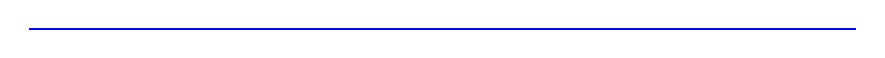
\begin{tikzpicture}
	\draw[thick, color=Blue] (0,0) -- (10.5,0);
	\end{tikzpicture}
\begin{itemize}
\item[\textbf{RE.1}] There are no perfect linear relationships among explanatory variables. [replaces \textcolor{Blue}{\textbf{FE.3}}]
\item[\textbf{RE.2}] In addition to \textcolor{Blue}{\textbf{FE.4}}, the expected value of $a_i$ given all regressors is constant: $E(a_i \mid \bm{X}_i)=\beta_0$. [Rules out correlation between $a_i$ and $\bm{X}_i$]
\item[\textbf{RE.3}] In addition to \textcolor{Blue}{\textbf{FE.5}}, variance of $a_i$ given all regressors is constant: $\textit{var}(a_i \mid \bm{X}_i)=\sigma^2_a$ [Homoskedasticity imposed on $a_i$]
\end{itemize}
\end{frame}
%---------------------------------
\begin{frame}{RE estimator – Assumptions}
Under  \textcolor{Blue}{\textbf{FE.1+FE.2+RE.1+(FE.4+RE.2)}}\\
RE estimator is consistent and asymptotically normal \\(for fixed $T$ as $N \rightarrow \infty$).\\
RE standard errors and statistics are not valid unless \textcolor{Blue}{\textbf{(FE.5+RE.3)}} and  \textcolor{Blue}{\textbf{FE.6}} conditions are met.\\
\bigskip
Under  \textcolor{Blue}{\textbf{FE.1-FE.2+RE.1+(FE.4+RE.2)+(FE.5+RE.3)+FE.6}}\\
RE estimator is consistent and asymptotically normal \\(for fixed $T$ as $N \rightarrow \infty$).\\
RE standard errors and statistics are valid.\\
RE is asymptotically efficient 
\begin{itemize}
\item[-] lower st.errs. than pooled OLS
\item[-] for time-varying variables, RE estimator is more efficient than FE (FE cannot be used on time-invariant variables).
\end{itemize}
\end{frame}
%---------------------------------
\begin{frame}{RE estimator – Example}
\textbf{Example:}\\
{\small \textbf{Wage equation using using panel data}}
\begin{align*}
\widehat{\log}(\textit{wage}_{it})
  = \ & .92 \  \mytikzmark{educ}{\boxed{\textit{educ}_{it}}} - 
       \textit{black}_{it} + \textit{hisp}_{it}      \\
( & .011)  \qquad \quad  (.048)  \qquad \quad \ (.043) \\
+ \ & .106 \ \textit{exper}_{it} - .0047 \ \textit{exper}^2_{it} + .064 \ \textit{married}_{it} \\
( & .015)  \qquad \quad \ \  (.0007)  \qquad \quad \ \ (.017) \\
+ \ & .106 \ \textit{union}_{it} +  \textit{time dummies} \\
( & .018)
\end{align*}
\begin{tikzpicture}[<-,overlay,remember picture,inner sep=1.5pt,shorten <=0.2em,font=\scriptsize]
\tikzset{
    mynode/.style={rectangle,draw=ProcessBlue, fill=White, semithick, inner sep=.2em, minimum size=2em, text centered, text width=10em},
    myarrow/.style={<-, >=stealth, thin, Red}
}
\node[mynode] at (9.4,5.3) (box){Random effects is used because many of the variables are time-invariant. \underline{But is the random effects} \underline{assumption realistic?}};
  \draw[myarrow] (educ) -- ++   (box);
\end{tikzpicture}

\textbf{Random effects or fixed effects?} \\
In economics, unobserved individual effects are rarely uncorrelated with explanatory variables. \\Hence, FE model/estimation is more convincing.
\end{frame}
%---------------------------------
\begin{frame}{RE vs FE estimator}
Hausman test / Hausman statistics may be used to choose between RE and FE: \\
$$H=(\hat{\bm{\beta}}_{FE} - \hat{\bm{\beta}}_{RE})^T [\widehat{\textit{Avar}}(\hat{\bm{\beta}}_{FE}) - \widehat{\textit{Avar}}(\hat{\bm{\beta}}_{RE})]^{-1} (\hat{\bm{\beta}}_{FE} - \hat{\bm{\beta}}_{RE}) \underset{H_0}{\sim} \chi^2(M)$$
{\footnotesize where $M$ is the number of regressors varying across $i$ and $t$.}
\bigskip
\begin{itemize}
\item[$H_0$:] $\textit{cov}(\bm{x}_{it},a_i) = 0$ \dots i.e. the crucial RE assumption holds
\item[$H_1$:] RE assumptions violated.
\end{itemize}
\end{frame}
%---------------------------------
\begin{frame}{RE vs FE estimator}
\
{\small $$H=(\hat{\bm{\beta}}_{FE} - \hat{\bm{\beta}}_{RE})^T [\widehat{\textit{Avar}}(\hat{\bm{\beta}}_{FE}) - \widehat{\textit{Avar}}(\hat{\bm{\beta}}_{RE})]^{-1} (\hat{\bm{\beta}}_{FE} - \hat{\bm{\beta}}_{RE}) \underset{H_0}{\sim} \chi^2(M)$$}\\
\bigskip
If $\hat{\bm{\beta}}_{FE}$ and $\hat{\bm{\beta}}_{RE}$ do not differ too much [or when the asymptotic variances are relatively large] we do not reject \textcolor{Blue}{$H_0$} \dots if we may assume RE assumptions hold, both RE and FE are consistent, and RE is efficient. For asymptotic variance estimators ($\widehat{\textit{Avar}}$), see Wooldridge (2010).\\ 
\bigskip
If we reject \textcolor{Blue}{$H_0$}, we need to assume that RE assumptions are violated $\rightarrow$ RE is not consistent [we use FE] \\
\underline{CRE may be used to test FE vs. RE (explained next)}.
\end{frame}
%---------------------------------
\section{Correlated random effects (CRE)}
\begin{frame}{CRE estimator}
Correlated Random Effects (CRE) estimator - a synthesis of the RE and FE approaches: 
\vspace{0.5cm}
\begin{itemize}
\item $a_i$ viewed as random, yet they can be correlated with $\bm{x}_{it}$.\\
\vspace{0.2cm}
Specifically, as $a_i$ do not vary over time, it makes sense to allow for their correlation with the time average of $x_{it}:\overline{x}_i = T^{-1} \sum^T_{t=1}x_{it}$
\vspace{0.2cm}
\item CRE allows for incorporation of time-invariant regressors (compare to FE).
\vspace{0.2cm}
\item CRE allows for convenient testing of FE vs. RE.
\end{itemize}
\end{frame}
%---------------------------------
\begin{frame}{CRE estimator}
CRE: The individual-specific effect $a_i$ is split up into a part that is related to the time-averages of the explanatory variables and a part $r_i$ (a time-constant unobservable) that is unrelated to the explanatory variables: 
\begin{align*}
\textnormal{For } y_{it} & =  \beta_1 x_{it} + a_i + u_{it}\textnormal{, we assume (a single-regressor illustration):}\\ \vspace{0.3cm}
a_i & = \alpha + \gamma \overline{x}_i + r_i \textnormal{, now: } \textit{corr}(r_i, \overline{x}_i) = 0 \Rightarrow \mytikzmark{corr}{\textit{corr}(r_i,x_{it})} = 0\\
\end{align*}
By substituting for $a_i$ into the first equation, we obtain: \\
$y_{it} = \alpha + \beta_1 x_{it} + \gamma \overline{x}_i + r_i + u_{it}$ \\
\bigskip
\underline{This equation can be estimated using RE}\\
As $\gamma \overline{x}_i$ controls for the correlation between $a_i$ and $x_{it}$, \\$r_i$ is uncorrelated with regressors.
\begin{tikzpicture}[<-,overlay,remember picture,inner sep=1.5pt,shorten <=0.2em,font=\scriptsize]
\tikzset{
    mynode/.style={rectangle,draw=ProcessBlue, fill=White, semithick, inner sep=.2em, minimum size=1em, text centered, text width=13em},
    myarrow/.style={->, >=stealth, thin, Red}
}
\node[mynode] at (3,3.1) (bcs){Because $\overline{x}_i$  is a linear function of  $x_{it}$};
\draw[myarrow] (bcs) -- ++   (corr);
\end{tikzpicture}
\end{frame}
%---------------------------------
\begin{frame}{CRE estimator}
CRE: \ $y_{it} = \alpha + \beta_1 x_{it} + \gamma \overline{x}_i + r_i + u_{it}$ \\
\medskip
\small CRE is a modified RE of the original equation $y_{it} =  \beta_1 x_{it} + a_i + u_{it}$: \\
\vspace{0.2cm}
with uncorrelated random effect $r_i$ but with the time averages as additional regressors. \\
\vspace{0.3cm}
\underline{The resulting CRE estimate for $\beta$ is identical to the FE estimator}.
\begin{itemize}
\item CRE allows for incorporation of time-invariant regressors: Besides $\hat{\beta}_{\textit{CRE}} = \hat{\beta}_{\textit{FE}}$, we can include arbitrary time invariant regressors and estimate $\gamma_{\textit{CRE}}$ values.
\item CRE allows for convenient testing of FE vs. RE:
	\begin{itemize}
	\item[$H_0$:] $\gamma = 0$ can be evaluated using $\hat{\gamma}_{\textit{CRE}}$ and appropriate (HCE) standard errors against
	\item[$H_1$:] $\gamma \neq 0$
	\end{itemize}
\end{itemize}
[RE assumes $\gamma = 0$: if we reject $H_0$, we also reject RE in favor of FE]
\end{frame}
%---------------------------------
\begin{frame}{CRE estimator}
The application of CRE to a model with multiple regressors is simple:
\begin{align*}
y_{it} & = \beta_1 x_{it1} + \dots + \beta_k x_{itk} + \circled{$a_i$} + u_{it},\ i = 1, \dots, N, \ t = 1, \dots, T \\
\bigskip
\circled{$a_i$} & = \alpha + \gamma_1 \mytikzmark{x1}{\circled{$\overline{x}_{i1}$}} + \dots + \gamma_k \mytikzmark{xk}{\circled{$\overline{x}_{ik}$}} + r_i\\
\end{align*}
\begin{tikzpicture}[<-,overlay,remember picture,inner sep=1.5pt,shorten <=0.2em,font=\scriptsize]
\tikzset{
    mynode/.style={rectangle,draw=White, fill=White, semithick, inner sep=0em, minimum size=0em, text centered, text width=20em},
    myarrow/.style={->, >=stealth, thin, Red}
}
\node[mynode] at (4,0.9) (0){Within means for all time-variant regressors};
  \draw[myarrow] (0) -- ++   (x1);
  \draw[myarrow] (0) -- ++  (xk);
\end{tikzpicture}
$$\Rightarrow y_{it} = \beta_0 + \alpha + \beta_1 x_{it1} + \dots + \beta_k x_{itk} + \gamma_1 \overline{x}_{i1} + \dots + \gamma_k \overline{x}_{ik} + [r_i + u_{it}]$$
\end{frame}
%---------------------------------
\section{Applying panel data methods to other data structures}
\begin{frame}{Applying panel data methods to other data structures}
\begin{itemize}
\item Panels are designed for two dimensional data.\\
(Data are grouped by both cross section and time period.) \\
\medskip
\item Grouping data is sometimes useful even when there is only one dimension to group along \\(clusters, matched pairs, countries, etc.). \\
\medskip
In other words, sometimes it’s useful to pretend that data come in a panel even when they don’t. \\
\medskip
\item This can be a useful tool for estimating separate intercepts for each group/cluster.
\end{itemize}
\end{frame}
%---------------------------------
\begin{frame}{Applying panel data methods to other data structures}
\textit{EViews Illustrated} example, based on data from the USA:\\
\small (Current Population Survey for March 2004; 100,000 individuals)\\
\vspace{0.5cm}
$\log(\textit{wage}_i) = \beta_0 + \beta_1 \textit{educ}_i + \beta_2 \textit{age}_i + \beta_3 \textit{asian}_i + u_i$\\
\vspace{0.5cm}
In pooled OLS, $\hat{\bm{\beta}}$ may be biased due to different wage levels (average wages) in different federal states. This may be controlled directly – by including dummies for the 51 states \dots \\
\vspace{0.5cm}
Often, it is more convenient to pretend that each state identifies a cross section in a panel. Then, we may use the FE/RE/CRE estimation ($a_s$ are the state-specific wage effects):\\
\vspace{0.5cm}
$\log(\textit{wage}_{si}) = \beta_0 + \beta_1 \textit{educ}_{si} + \beta_2 \textit{age}_{si} + \beta_3 \textit{asian}_{si} + a_s + u_{si}$
\end{frame}
%---------------------------------
\section{Autocorrelation \& heteroskedasticity in panel data models}
\begin{frame}{Autocorrelation and heteroskedasticity in panel data models}
\underline{\textbf{Panel data extensions:}} \qquad  $y_{it} = \bm{x}_{it} \bm{\beta} + a_i + u_{it}$\\
\bigskip
\underline{Heteroskedasticity} \\
$\textnormal{RE model:~} \ \textit{var}(v_{it} \mid \bm{X}_i) = \sigma^2_{a_i} + \textit{var}(u_{it} \mid \bm{X}_i) = \Bigg\{ \parbox{2cm}{$\sigma^2_{a_i} + \boxed{\sigma^2_{u_i}} \\ \sigma^2_{a_i} + \boxed{\sigma^2_{u_{t}} }$}$\\
\bigskip
{\small \underline{Correlation between cross-sectional units (contemporaneous correlation)}} \\
\medskip
{\small The general $H_0$ of no C-S dependence may be written as follows:} \\
$$\rho_{ij} = \textit{corr}(u_{it}, u_{jt}) = 0 \textit{ \ for \ } i \neq j$$
\end{frame}
%---------------------------------
\begin{frame}{Autocorrelation \& heteroskedasticity in panel data models}
\underline{\textbf{Panel data extensions:}} \qquad  $y_{it} = \bm{x}_{it} \bm{\beta} + a_i + u_{it}$\\
\bigskip
\underline{Serial correlation (between-period correlation)} \\
\smallskip
$u_{it} = \Bigg\{ \parbox{5cm}{$\boxed{\rho \ } u_{i,t - 1} + \varepsilon_{it} \\ \boxed{\rho_i} u_{i,t - 1} + \varepsilon_{it} $}$\\
\bigskip
\underline{Non-stationarity and panel cointegration} \\
\medskip
For the above  ``extensions'', tests and GLS methods are usually estimator-specific (FD/FE/RE/CRE). Different types of assumption violations may occur simultaneously. Topic not covered in this course, see e.g. Wooldridge, 2010 for details.
\end{frame}
%---------------------------------
\section{Arellano-Bond estimator (dynamic panels)}
\begin{frame}{Arellano-Bond estimator (dynamic panels)}
Dynamic panel\\
\medskip
$y_{it} = \delta_1 y_{i,t-1} + \bm{x}^{\prime}_{it} \bm{\beta} + a_i + u_{it}$\\
\medskip
\dots May be expanded using additional lags of the dependent variable or using lagged exogenous regressors.\\
\medskip
\small
\textbf{Nickel Bias}
\begin{itemize}
\item Related mostly to the lagged exogenous regressors $\bm{x}$
\item FEs take up some part of the dynamic effect and therefore dynamic panel data models lead to overestimated FEs and underestimated dynamic interactions. 
\item Whether the Nickel bias is significant in a particular model/dataset situation is an empirical question. Nevertheless, in theory this bias persists unless the number of time observations goes to infinity.
\item The inclusion of additional cross-sections to the dataset would worsen the bias in most cases.
\end{itemize}
\end{frame}
%---------------------------------
\begin{frame}{Arellano-Bond estimator (dynamic panels)}
\textbf{Arellano-Bond} (AB) \textbf{estimator} 
\begin{itemize}
\item The model is transformed into first differences to eliminate the individual effects:\\
$\Delta y_{it} = \delta_1 \Delta y_{i,t-1} + \Delta \bm{x}^T_{it} \bm{\beta} + \Delta u_{it}$, 
\item then a generalized method of moments (GMM) approach is used to produce asymptotically efficient estimates for the dynamic coefficients.
\item AB approach is based on IV (we need instruments for the lagged dependent variable – this is an endogenous regressor, correlated with the errors in the FD model).
\item \textcolor{Red}{Warning:} AR(2) / not AR(1) / autocorrelation in residuals of the AB-estimated model renders the AB estimator inconsistent. After using the AB estimator, always test for AR(2) autocorrelation in the residuals!
\end{itemize}
\end{frame}
%---------------------------------
\section{Panel data - Extensions}
\begin{frame}{Panel data - Extensions}
\begin{itemize}
\item Advanced course on panel data \\
\textsubscript{\textcolor{Blue}{\url{http://people.stern.nyu.edu/wgreene/Econometrics/PanelDataNotes.htm}} }
\bigskip
\item Mixed effects model \\
Extension to the RE model \\(intercept and -some- coefficients have a random term):
$$
y_{it}=\bm{x}_{it}^{\prime} \bm{\beta} + \bm{z}_{it}^{\prime}( \bm{\gamma} + \bm{h}_i) +
(\alpha + u_i) + \varepsilon_{it}
$$
where $\bm{h}_i$ describes random variation of the paremeter(s) across individuals.\\
\medskip

\textsubscript{ \textcolor{Blue}{\url{http://www.bodowinter.com/tutorial/bw_LME_tutorial1.pdf}} } \\
\end{itemize}
\end{frame}
%---------------------------------
\end{document}